\item \textbf{{[}PJC/PRELIM/9597/2015/P1/Q3{]} }

A program is to be written to find all the words in a piece of text
and to print them in alphabetical order, together with the number
of times each word occurs. The data structure used to hold this information
will be a linked list, with each node holding a word, the number of
occurrence of that word, and a pointer to the node containing the
next word in alphabetical order. 

The program will use nodes implemented as instances of the class ListNode.
The class \texttt{ListNode} has the following properties: 
\noindent \begin{center}
\begin{tabular}{|l|l|l|}
\hline 
\multicolumn{3}{|c|}{\texttt{Class: ListNode}}\tabularnewline
\hline 
\multicolumn{3}{|c|}{Properties}\tabularnewline
\hline 
\texttt{\hspace{0.01\columnwidth}}Identifier & \texttt{\hspace{0.01\columnwidth}}Data Type & \texttt{\hspace{0.05\columnwidth}}Description\tabularnewline
\hline 
\texttt{Word} & \texttt{STRING} & The node\textquoteright s value for a word from the text \tabularnewline
\hline 
\texttt{Count} & \texttt{INTEGER} & The node's value for number of occurrences of the word\tabularnewline
\hline 
\texttt{Pointer} & \texttt{INTEGER} & The pointer for the node\tabularnewline
\hline 
\end{tabular}
\par\end{center}

A linked list is implemented as an instance of the class \texttt{LinkedList}.
The class \texttt{LinkedList} has the following properties and methods: 
\noindent \begin{center}
\begin{tabular}{|l|l|l|}
\hline 
\multicolumn{3}{|c|}{\texttt{Class: LinkedList}}\tabularnewline
\hline 
\multicolumn{3}{|c|}{Properties}\tabularnewline
\hline 
\texttt{\hspace{0.01\columnwidth}}Identifier & \texttt{\hspace{0.01\columnwidth}}Data Type & \texttt{\hspace{0.05\columnwidth}}Description\tabularnewline
\hline 
\texttt{Node} & \texttt{ARRAY{[}30{]} of ListNode} & The linked list data structure -- data values (Word \& Count) and
pointers. Array index starts at 0. For testing purposes, the dataset
has a maximum of 30 nodes. \tabularnewline
\hline 
\texttt{Start} & \texttt{INTEGER} & Index position of the node at the start of the linked list\tabularnewline
\hline 
\texttt{NextFree} & \texttt{INTEGER} & Index position of the next unused node\tabularnewline
\hline 
\end{tabular}
\par\end{center}

\noindent \begin{center}
\begin{tabular}{|l|l|l|}
\hline 
\multicolumn{3}{|c|}{\texttt{Class: LinkedList}}\tabularnewline
\hline 
\multicolumn{3}{|c|}{Methods}\tabularnewline
\hline 
\texttt{\hspace{0.01\columnwidth}}Identifier & \texttt{\hspace{0.01\columnwidth}}Data Type & \texttt{\hspace{0.05\columnwidth}}Description\tabularnewline
\hline 
Initialise & PROCEDURE & Sets all node data values to empty string (for Word) and 0 (for Count).
Set pointers to indicate all nodes are unused and linked. Initialise
values for Start and NextFree.\tabularnewline
\hline 
Update & PROCEDURE & Updates the linked list with a word read from the text\tabularnewline
\hline 
Display & PROCEDURE & Display the current state of array content and pointers in table form.\tabularnewline
\hline 
IsEmpty & FUNCTION RETURNS BOOLEAN & Test for empty linked list.\tabularnewline
\hline 
IsFull & FUNCTION RETURNS BOOLEAN & Test for no unused nodes.\tabularnewline
\hline 
\end{tabular}
\par\end{center}

The diagram shows the linked list with: 
\begin{itemize}
\item the text \textquotedblleft mary had a little lamb\textquotedblright{}
added 
\item the unused nodes linked together. 
\end{itemize}
\begin{center}
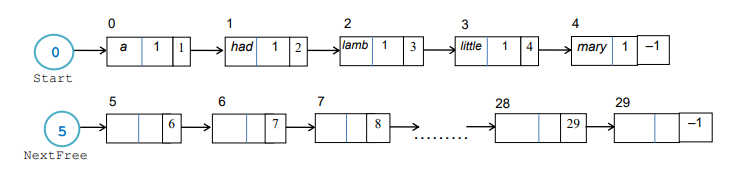
\includegraphics[width=0.65\paperwidth]{C:/Users/Admin/Desktop/Github/question_bank/LyX/static/img/9597-PJC-2015-P1-Q3-1}
\par\end{center}

\subsection*{Task 3.1}

Write the program code for the classes \texttt{ListNode} and \texttt{LinkedList},
including the \texttt{Initialise}, \texttt{Display}, \texttt{IsEmpty}
and \texttt{IsFull} method. The code should follow the specification
given. Do not write the \texttt{Update} procedure yet. 

\subsection*{Evidence 10: }

Your program code for the \texttt{ListNode} and \texttt{LinkedList}
classes. \hfill{}{[}12{]}

\subsection*{Task 3.2}

Write code to create a \texttt{LinkedList} object and run \texttt{Display}
procedure to show the content of the object. 

\subsection*{Evidence 11: }

Screenshot confirming all values after initialisation of the \texttt{LinkedList}.\hfill{}
{[}3{]}

\subsection*{Task 3.3 }

Write code to implement for the \texttt{LinkedList} class the \texttt{Update}
method that will update the linked list with a word read from the
text. 

\subsection*{Evidence 12:}

Program code for \texttt{Update} procedure. \hfill{}{[}12{]}

\subsection*{Task 3.4 }

Write code to use the Update procedure by reading in the text from
the file \texttt{Story.txt}. 

\subsection*{Evidence 13:}

Screenshot of state of array content and pointers by running \texttt{Display}
procedure. \hfill{}{[}4{]}

\subsection*{Task 3.5 }

Write a method \texttt{Query} inside \texttt{LinkedList} class that: 
\begin{itemize}
\item takes a word input by user, 
\item check if the word exists in the linked list, 
\item output appropriate message with the number of occurrences, if word
exists.
\end{itemize}

\subsection*{Evidence 14: }

Program code for \texttt{Query} method. \hfill{}{[}4{]}

\subsection*{Evidence 15: }

Screenshot from running the \texttt{Query} method for a word that
exists and another word that does not exist in the linked list. \hfill{}{[}2{]}